%%%%%%%%%%%%%%%%%%%%%%%%%%%%%%%%%%%%%%%%%%%%%%%%%%%%%%%%%%%%%%%%%%% 
%                                                                 %
%                            CHAPTER                              %
%                                                                 %
%%%%%%%%%%%%%%%%%%%%%%%%%%%%%%%%%%%%%%%%%%%%%%%%%%%%%%%%%%%%%%%%%%% 
 
\chapter{Implementation}
In this chapter, we will discuss the implementation of the network. We will first discuss the dataset and network architecture we will be using. We will then go into detail about the implementation of the network and the training process. 

\section{Dataset}
In this section, we will go over the datasets used in this paper, both the datasets used to pretrain the models and the few-shot shell dataset we are introducing ourselves.

\subsection{COCO}

Microsoft's Common Objects in Context (COCO) dataset is a large-scale object detection and segmentation dataset. It contains 330K images with 1.5M instance annotations of 80 different classes. It is split into a training set of 118K images, a validation set of 5K images and a test set of 40K images(the other images are unlabeled). \citet{COCO}

\subsection{Shells}

The shell dataset is a new dataset we are introducing ourselves. The images were taken with a cellphone camera on the Belgian coast. Each image has a size of 6144x8192px. Due to limited resources, the dataset is quite small, containing only 96 annotated images and 206 unannotated images. The images are annotated with bounding boxes of 8 types of shells, with 614 annotations in total. An overview of the annotations per class can be found in table \ref{tab:shell_annotations}. The images are mostly sparse, with 1 to 3 shells per image. Some denser images are also present however. A graph of the annotations per image in the dataset can be found in figure \ref{fig:annotations_per_img}. Some examples of the images in the dataset can be found in table \ref{tab:shell_examples}.

%annotations: {
%     "Baltic tellin": 69,
%     "Cockle": 89,
%     "Thick trough shell": 91,
%     "Mussel": 268,
%     "Banded wedge shell": 32,
%     "Elliptical trough shell": 18,
%     "Cut trough shell": 36,
%     "Oyster": 9
% }

\begin{table}[h]
    \centering
    \captionsetup{justification=centering}
    \begin{tabular}{|l|l|}
    \hline
    \textbf{Shell type} & \textbf{Number of annotations} \\ \hline
    Baltic tellin       & 69                             \\ \hline
    Cockle              & 89                             \\ \hline
    Thick trough shell  & 91                             \\ \hline
    Mussel              & 268                            \\ \hline
    Banded wedge shell  & 32                             \\ \hline
    Elliptical trough shell & 18                         \\ \hline
    Cut trough shell    & 36                             \\ \hline
    Oyster              & 9                              \\ \hline
    \end{tabular}
    \caption{Overview of the annotations per class in the shell dataset.}
    \label{tab:shell_annotations}
\end{table}

\begin{figure}[h]
    \centering
    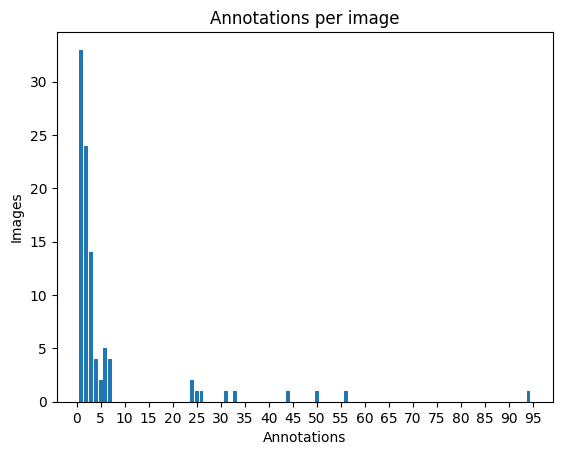
\includegraphics[width=0.8\textwidth]{chapter3/annotations_per_img.png}
    \caption{Overview of the annotations per image in the shell dataset.}
    \label{fig:annotations_per_img}
\end{figure}

\begin{table}[h]
    \centering
    \captionsetup{justification=centering}
    \begin{tabular}{|c|c|c|}
    \hline
    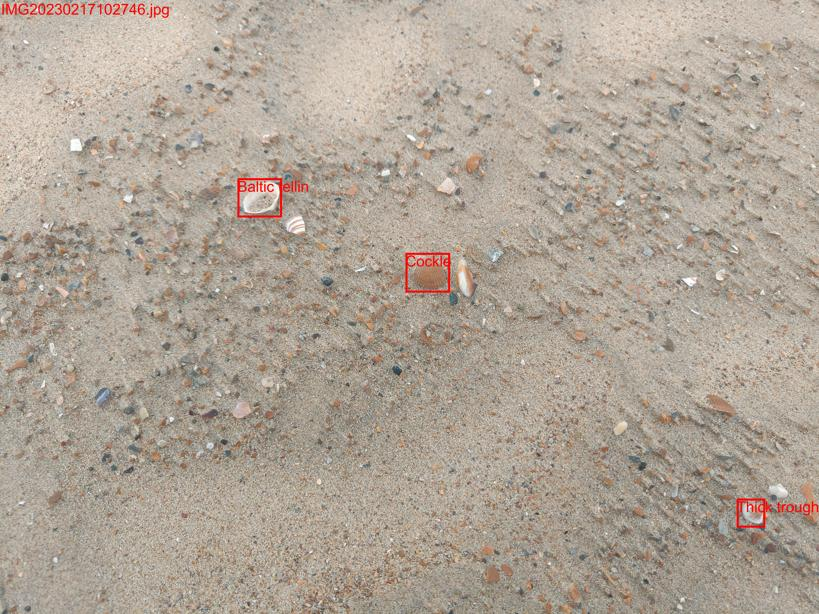
\includegraphics[width=0.3\textwidth]{chapter3/shell_examples/1.jpg} & 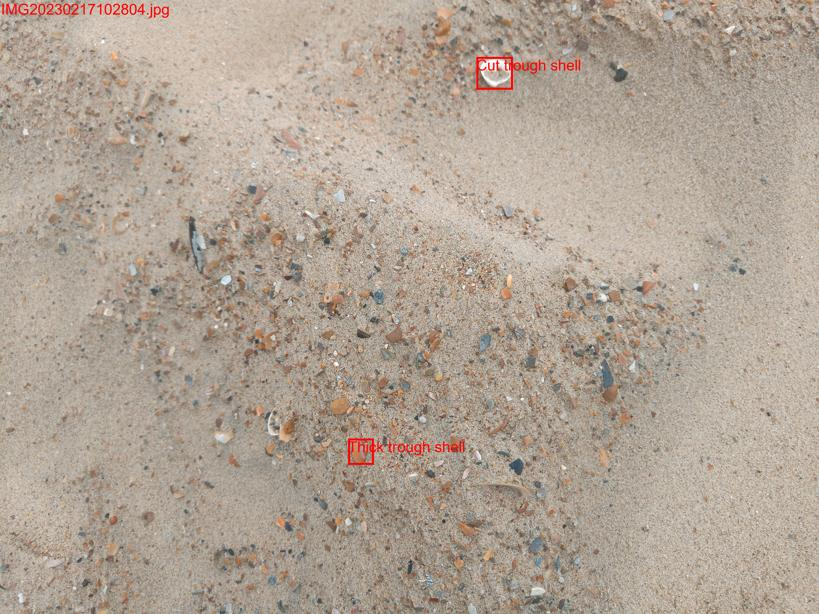
\includegraphics[width=0.3\textwidth]{chapter3/shell_examples/2.jpg} & 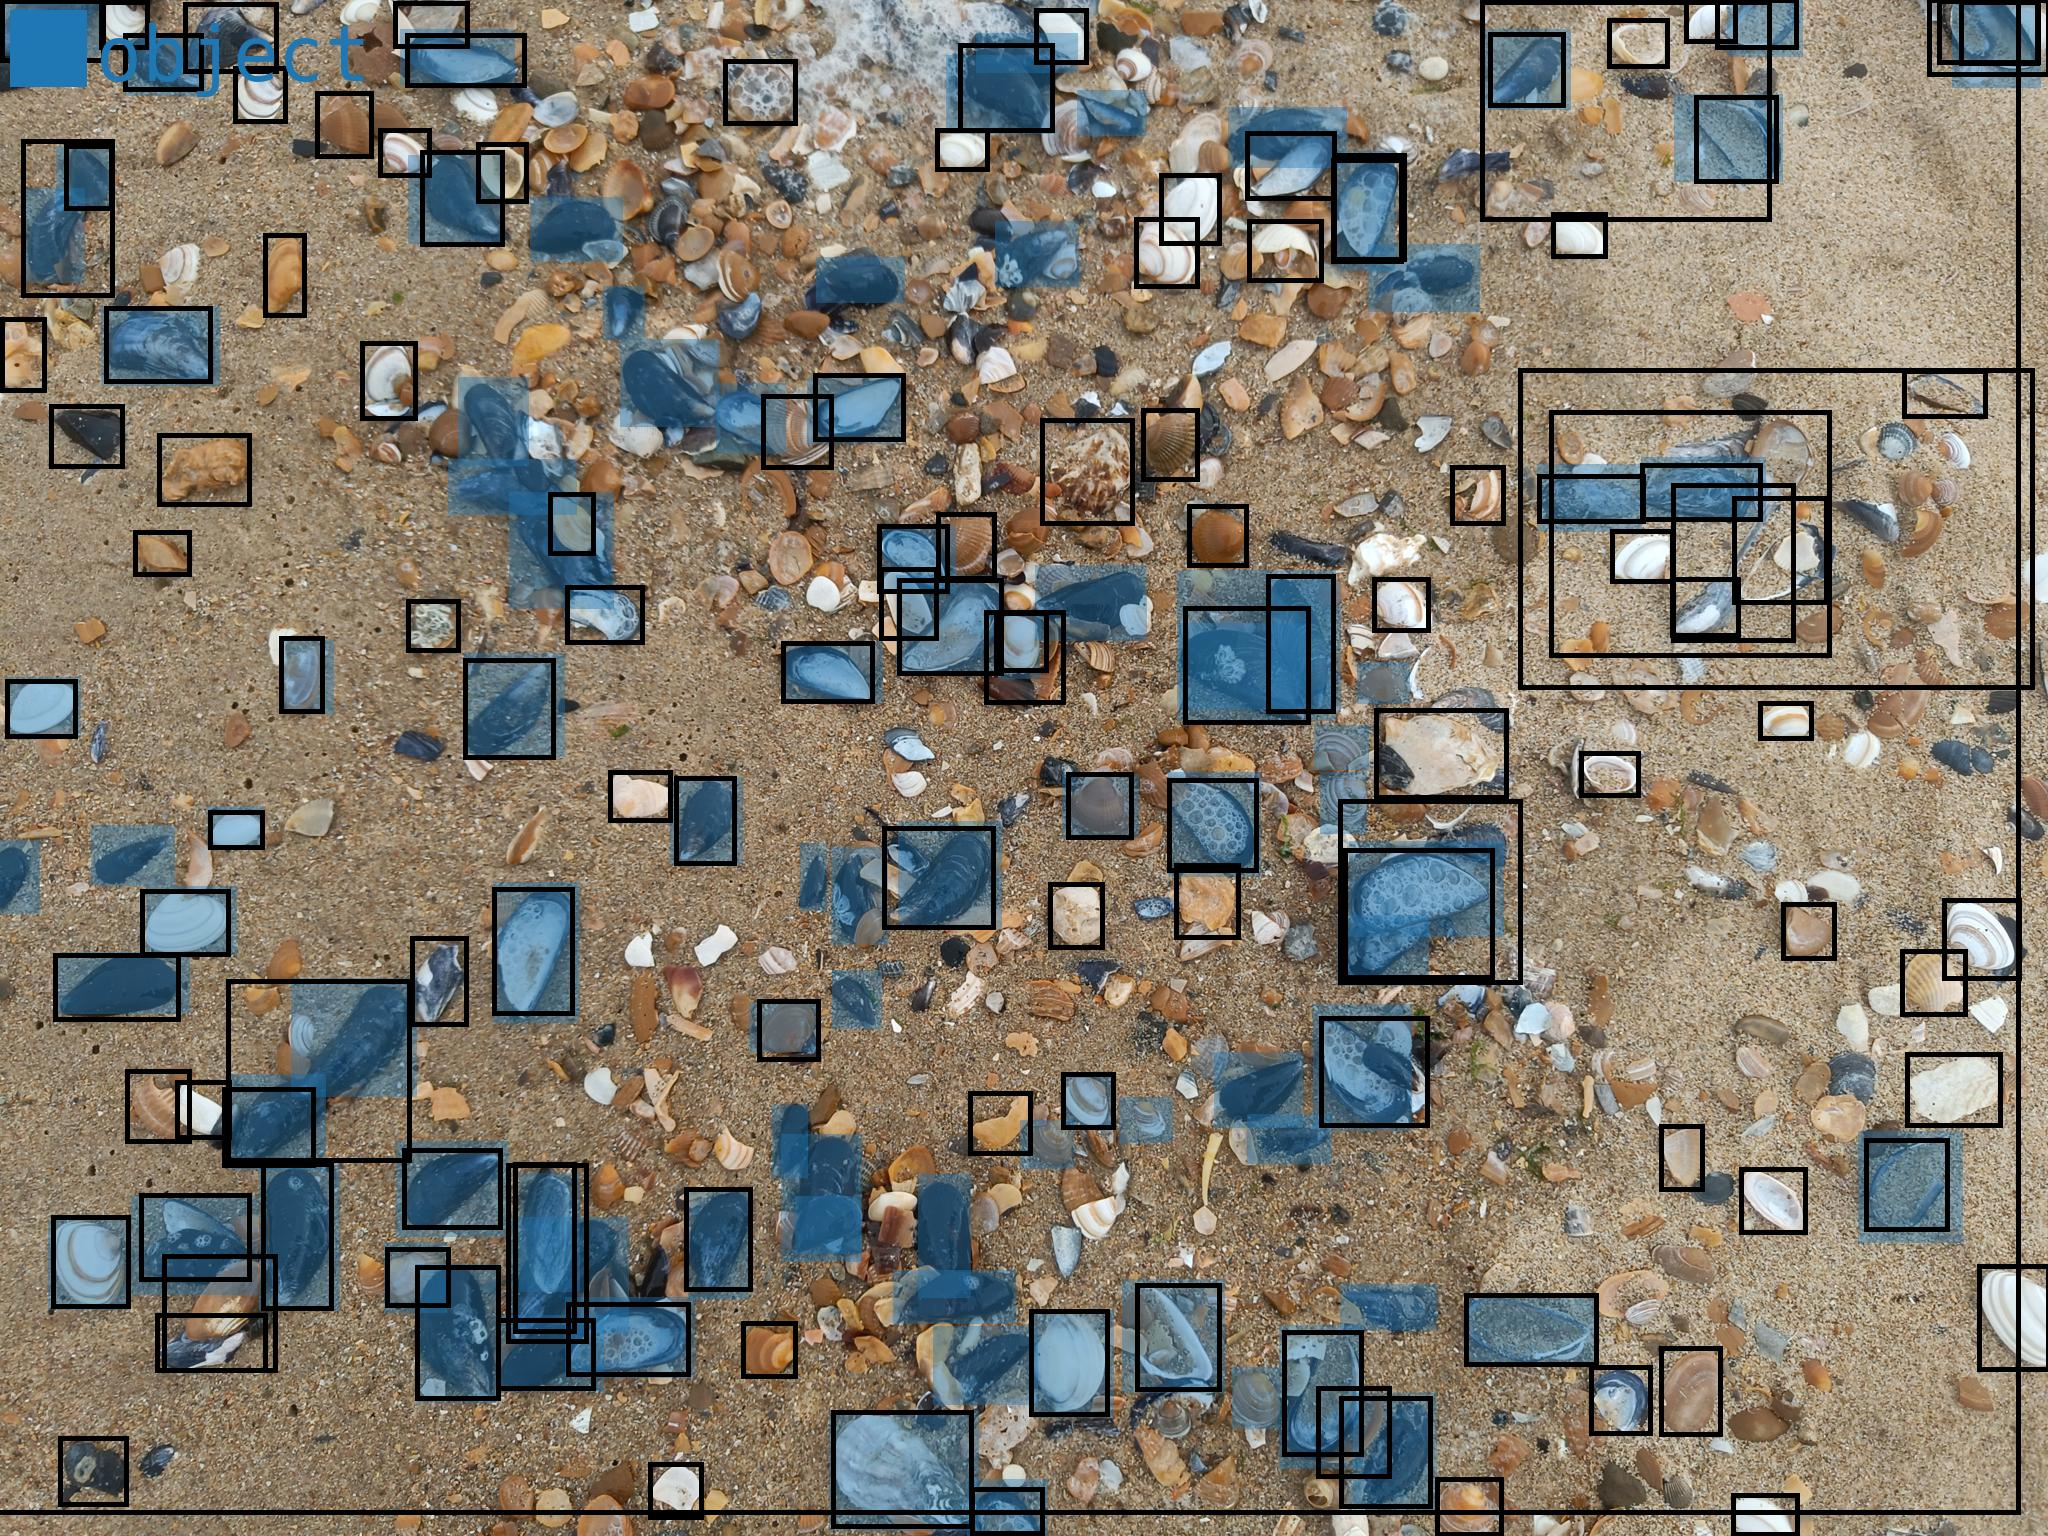
\includegraphics[width=0.3\textwidth]{chapter3/shell_examples/3.jpg} \\ \hline
    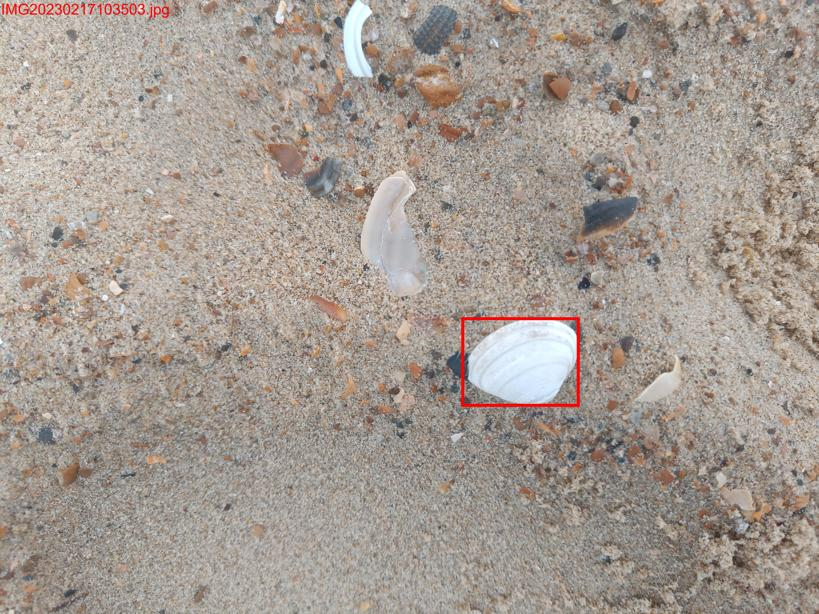
\includegraphics[width=0.3\textwidth]{chapter3/shell_examples/4.jpg} & 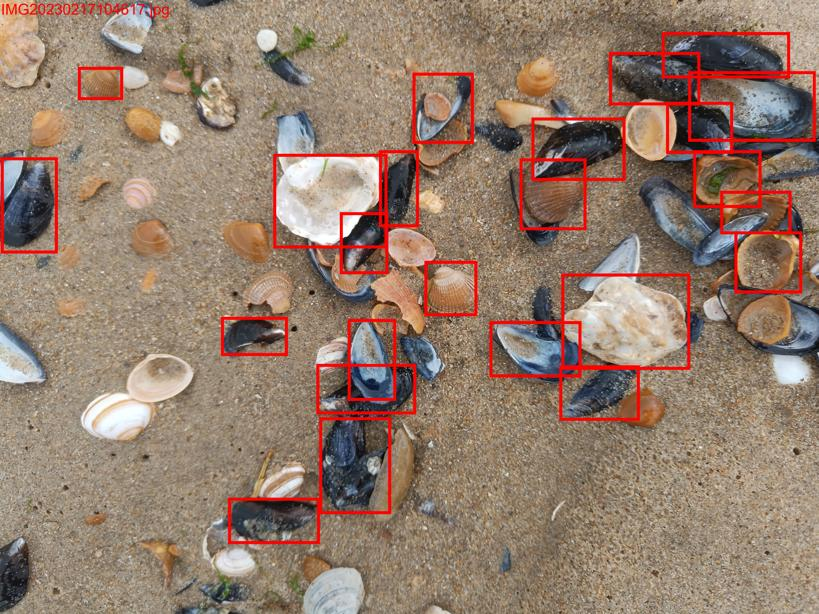
\includegraphics[width=0.3\textwidth]{chapter3/shell_examples/5.jpg} & 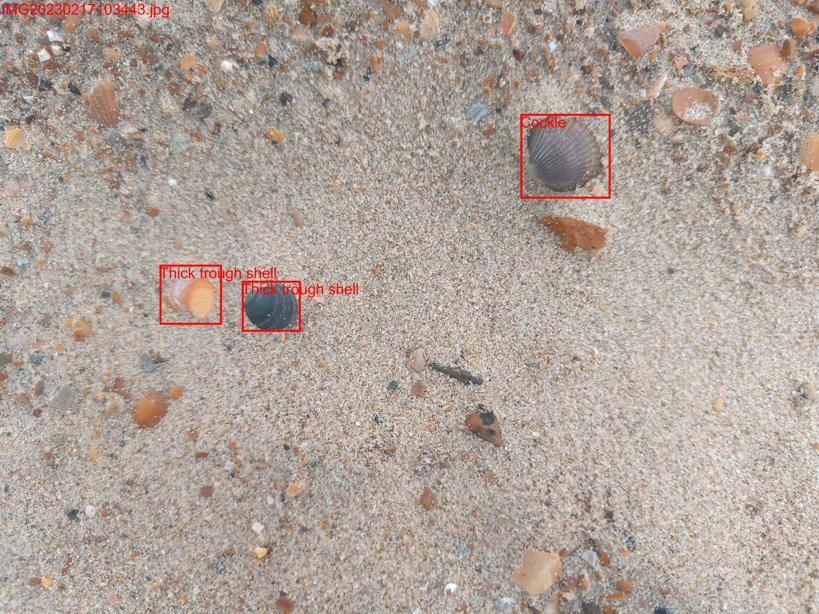
\includegraphics[width=0.3\textwidth]{chapter3/shell_examples/6.jpg} \\ \hline
    \rotatebox{90}{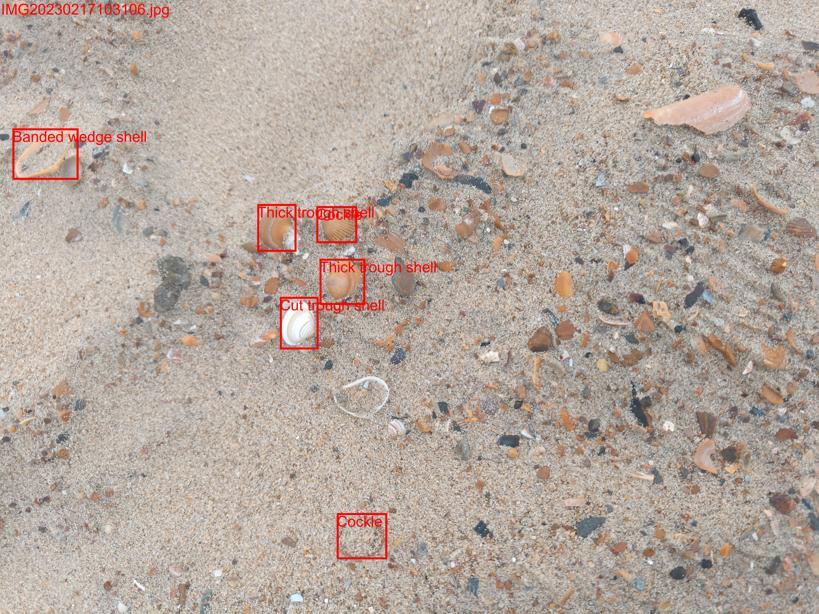
\includegraphics[height=0.3\textwidth]{chapter3/shell_examples/7.jpg}} & \rotatebox{90}{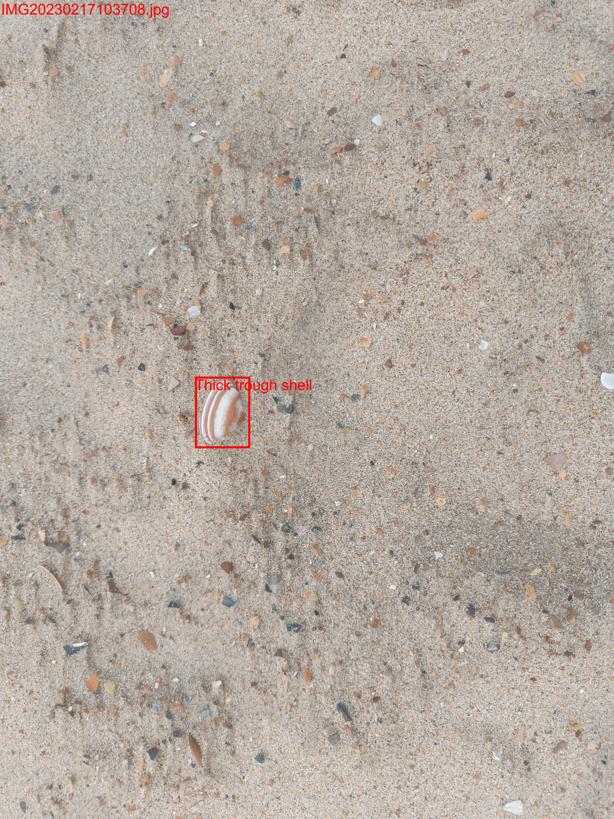
\includegraphics[height=0.3\textwidth]{chapter3/shell_examples/8.jpg}} & \rotatebox{90}{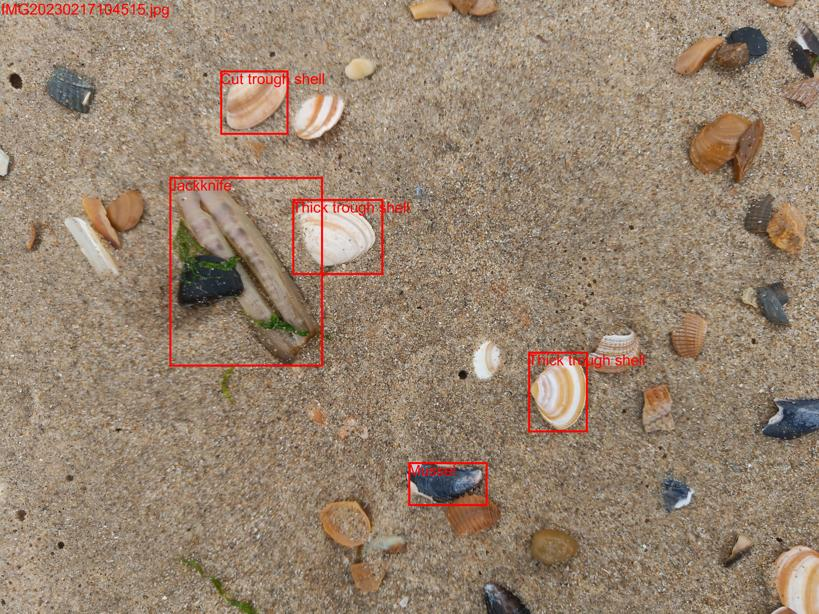
\includegraphics[height=0.3\textwidth]{chapter3/shell_examples/9.jpg}} \\ \hline
    \end{tabular}
    \caption{Examples of images in the shell dataset.}
    \label{tab:shell_examples}
\end{table}


